\chapter{Design}\label{cha:design}
This chapter will cover the design of the solution, in particular focusing on the following areas:

\begin{itemize}
	\item Required Features
	\item Languages, Technologies and Frameworks
	\item Architecture
\end{itemize}

The design phase aims to ensure that the limited development time available prioritises the most effective features.

\section{MoSCoW Requirements}

Before considering specific technologies and frameworks, a list of MoSCoW requirements is produced, shown in the table below. The first column represents whether the requirement is \textbf{F}unctional or \textbf{N}on-\textbf{F}unctional, and the second column represents requirements that \textbf{M}ust, \textbf{S}hould or \textbf{C}ould be completed.

\begin{center}
	\begin{xltabular}{0.82\paperwidth}{ | p{1.5cm} | p{1.5cm} | X | } 
		\hline
		\textbf{F / NF} & \textbf{Priority} & \textbf{Requirement Description} \\ \hline
		
 		\multicolumn{3}{|c|}{Domain Specific Language - Expressions} \\ \hline
		F & M & The language must support 5 data types: integers, floats, booleans, strings and date-time objects. \\ \hline
		F & M & The language must be able to tolerate null values within a dataset. \\ \hline
		F & M & The language must allow users to reference a field in the current dataset. \\ \hline
		F & M & The language must allow users to reference a constant value, which can take one of the data types defined above. \\ \hline
		F & M & The language must support arithmetic operations like add, subtract, multiply, division and modulo. \\ \hline
		F & M & The language must support string slicing and concatenation. \\ \hline
		F & S & The language should utilise polymorphism in add operations to apply string concatenation, or arithmetic addition depending on the data types of the arguments. \\ \hline
		F & C & The language could be designed in such a way to allow the user to define their own functions. \\ \hline
		NF & S & The language should be intuitive to use, with SQL-like syntax. \\ \hline
		\multicolumn{3}{|c|}{~} \\ \hline
		\multicolumn{3}{|c|}{Domain Specific Language - Comparisons} \\ \hline
		F & M & The user must be able to provide expressions as inputs to comparison operators. \\ \hline
		F & M & The language must support equals, and not equals comparisons. \\ \hline
		F & M & The language must support inequalities, using numerical ordering for number types, and lexicographic ordering for strings. \\ \hline
		F & M & The language must support null and not null checks. \\ \hline
		F & S & The language should support string comparisons, including case sensitive and insensitive versions of contains, starts with, and ends with. \\ \hline
		F & S & The language should allow the user to combine multiple comparison criteria using $AND$ and $OR$ operators. \\ \hline
		
		\multicolumn{3}{|c|}{Data Processing} \\ \hline
		F & M & The system must allow users to apply Select operations on datasets, applying custom expressions to the input data. \\ \hline
		F & M & The system must allow users to apply Filter operations on datasets, applying custom comparisons to the input data. \\ \hline
		F & M & The system must allow users to apply Group By operations on datasets, which take expressions as unique keys, and aggregate operations to compute over the unique keys. \\ \hline
		F & M & The Group By operation must allow users to apply Minimum, Maximum, Sum and Count aggregate functions to Group By operations. \\ \hline
		F & C & The system could allow users to apply Distinct Count, String Concatenation, and Distinct String Concatenation aggregate functions to Group By operations. \\ \hline
		F & C & The system could allow users to join two datasets together according to custom criteria. \\ \hline
		NF & S & The complexities of the system should be hidden from the user; from their perspective the operation should be identical whether the user is running the code locally or over a cluster. \\ \hline
		
		\multicolumn{3}{|c|}{Cluster} \\ \hline
		F & M & The system must allow the user to upload source data to a permanent data store. \\ \hline
		F & M & The orchestrator node must split up the full query and delegate partial work to the worker nodes. \\ \hline
		F & M & The orchestrator node must collect partial results from the cluster nodes to produce the overall result for the user. \\ \hline
		F & M & The orchestrator node must handle worker node failures and other computation errors by reporting them to the user. \\ \hline
		F & S & The orchestrator should perform load balancing to ensure work is evenly distributed among all nodes. \\ \hline
		F & C & The orchestrator could handle worker node failures by redistributing work to active workers. \\ \hline
		F & M & The worker nodes must accept partial work, compute and return results to the orchestrator. \\ \hline
		F & M & The worker nodes must pull source data from the permanent data store. \\ \hline
		F & M & The worker nodes must report any computation errors to the orchestrator. \\ \hline
		F & S & The worker nodes should cache results for reuse in later queries. \\ \hline
		F & S & The worker nodes should spill data to disk storage when available memory is low. \\ \hline
		NF & S & The permanent data store should be chosen to provide performance benefits when importing source data. \\ \hline
	\end{xltabular}
\end{center}

\section{Language}
The first key design decision was to determine what languages would be used to implement the system. A decision was made to use more than one language, because the requirements of the user interface suit a different type of language to the other components.

\subsection{Frontend}\label{subsec:frontend-design}
The most important requirement for the frontend was to use SQL-like syntax. Pure SQL requires a text parser to generate queries, which would add a significant amount of development time to implement, so a language which would be able to encode queries as classes and functions was preferred. Python is an object-oriented language with these capabilities, and was therefore selected \cite{python3-10}. Furthermore, according to the 2022 StackOverflow Developer Survey, it is the fourth most popular programming language, supporting two of the most popular data processing frameworks: NumPy and pandas \cite{stackoverflowsurvey2022, reback2020pandas, harris2020array}. This popularity means that it is likely the widest range of users will have prior experience with Python, and there is the possibility of integrating with these frameworks to further improve the system's usability. 

\subsection{Orchestrator and Worker Nodes}
It was decided that the orchestrator and worker nodes will use the same language, as feature overlap between the two is likely. A language with either automatic or manual garbage collection (GC) had to be chosen. Manual GC would theoretically allow for higher performance due to more granular control over memory allocation. However, this could slow development, as time would have to be spent writing code to perform this process. Therefore, manually GC languages were ruled out.

The remaining options were a range of object-oriented and functional languages. Much of the project would be CPU intensive iteration over large lists of items, so a language with strong support for parallelisation was preferable. This ruled out languages like Python and JavaScript where parallelisation requires manual implementation by the developer \cite{pythonmultiprocessing, nodeworkerthreads}.

In the end, Scala was chosen \cite{scaladocs}. It features a mix of both object-oriented and functional paradigms, which would allow the best option to be selected for each task. Furthermore, Scala has built-in support for parallelisation through operations like $map$ and $reduce$, which is  helpful for iterating over or combining a dataset. It compiles into Java, meaning that Java packages can be executed in Scala, which proved useful for later design decisions \cite{scalaforjavadevs}.
 
\section{Runtime}
\subsection{Containerisation}
With this being a distributed systems project, the clear choice for executing the code was within containers. Docker is the best option for creating and executing containers, but is not suitable for running and managing large numbers of containers \cite{orchestrationdockerdocs}. For this, a container orchestration tool is required, where there are two main options: Docker Swarm, and Kubernetes \cite{dockerswarm, k8sapi}. Docker Swarm is closely integrated within the Docker ecosystem, but many cloud providers feature fully managed Kubernetes services, so Kubernetes was chosen.

\subsection{Network Communication} 
A framework had to be selected to allow the frontend, orchestrator and worker nodes to communicate. RPC frameworks are designed to implement custom function calls over a remote network, making them an excellent option to implement a custom query model \cite{srinivasan1995rpc}. The chosen framework was gRPC, designed and maintained by Google \cite{gRPCapi}. There are well-maintained drivers for Python and Scala, and gRPC uses protocol buffers (protobuf) as its message system, which are designed to be more space efficient than XML or JSON \cite{scalapbdocs, protobufdocs}. This would be useful for transmitting large amounts of data. 


\section{Persistent Storage}
There are a wide range of options for persistent data storage. The first key decision was whether to design a custom solution, or use an existing solution. A custom implementation would come with the benefit of being more closely integrated with the rest of the system, at the cost of increased development time. A decision was made not to create a custom solution due to time constraints, so a number of types of existing file systems and databases were instead considered, but were also not selected:
\begin{itemize}
	\item Single System SQL Databases \textit{(Microsoft SQL Server, PostgreSQL, MySQL)}: while this option would be fastest to start using due to extensive industry support, the database would quickly become a bottleneck, as all nodes would import data from the same location.
	\item Distributed File Systems \textit{(Hadoop Distributed File System)}: these provide a mechanism for storing files resiliently across a number of machines, removing the data import bottleneck. However, they provide no way of querying the stored data, so this feature would have to be implemented manually.
	\item Distributed NoSQL Databases \textit{(MongoDB, CouchDB)}: these spread the load of reading the data across a number of machines. However, the expected input data is tabular, meaning the NoSQL architecture is likely to result in added complexity when importing data.
\end{itemize}

\subsection{Apache Cassandra}\label{subsec:cassandra-design}
Apache Cassandra was chosen as the persistent storage mechanism for a number of reasons \cite{lakshman2010cassandra}. Firstly, the data model is tabular, as is the expected input data. Furthermore, Cassandra is a distributed database, so the source data will be stored across a number of nodes. This will increase the effective read speed when retrieving data, as the full load will be spread between the nodes.

\paragraph{Partitioning}
Cassandra's method of partitioning data is another key reason why it was selected. When a record is inserted into the database, Cassandra hashes the primary key, producing a 64-bit token. Each node in the database is assigned part of the full token range, which determines what records it holds \cite{lakshman2010cassandra}. Figure \ref{fig:cassandra-token-distribution} demonstrates how the full range of tokens is distributed among a number of Cassandra nodes.

\begin{figure}[h]
	\centering
	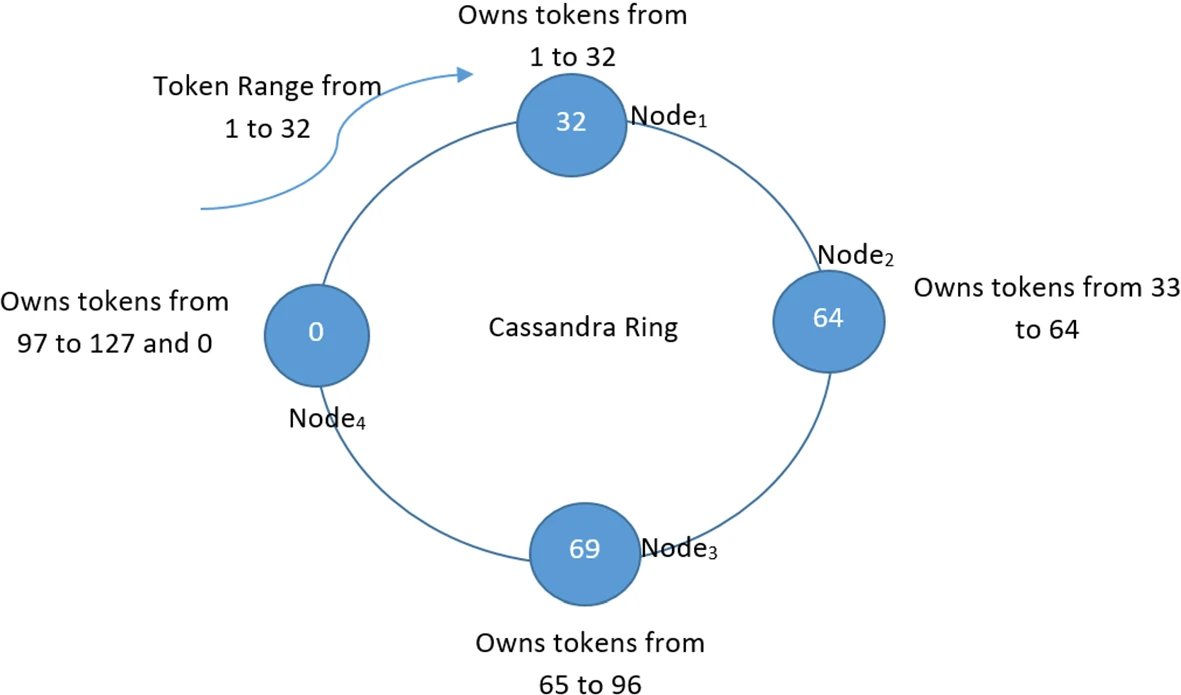
\includegraphics[width=0.5\textwidth]{chapters/diagrams/design/cassandra-token-distribution}
	\caption{Cassandra Token Ring Distribution \protect\cite{khatibi2019dynamic}}
	\label{fig:cassandra-token-distribution}
\end{figure}

Cassandra allows token ranges to be provided as filters in queries,  meaning the worker nodes can split up and control the data they read from the database, to read smaller chunks. 

\paragraph{Data Co-Location} Cassandra can be run on Kubernetes using K8ssandra \cite{k8ssandra}. This is particularly useful because the Cassandra cluster can be configured to run on the same machines as the worker nodes, enabling the source data to be co-located with the workers performing the computation. This decision meets the requirement to exploit the integration between the storage mechanism and cluster nodes, as data co-location will reduce the network latency when importing the source data, and increase transfer speed in some cases if the data never leaves the physical machine.

\paragraph{Language-Specific Drivers} Drivers for both Python and Java are available, which provide basic functionality for querying the database \cite{datastaxjavadriver, datastaxpythondriver}. There are optional modules for these drivers, and Scala-specific frameworks with more complex features, but these were not used as the extra functionality was not required, and the added complexity had the potential to cause problems. 

\section{Architecture}\label{sec:architecture}
Based on the above design choices, a high-level diagram was produced, detailing each of the system's components and the interaction between them, shown in Figure \ref{fig:overall-architecture}. The user will be able to define queries using the Python frontend, which are then sent using gRPC to the orchestrator. It will break the full query up into partial queries, which will be computed on the worker nodes. When the computation is complete, the workers will return results to the orchestrator, which will combine the result and return it to the frontend.

\begin{figure}[h]
	\centering
	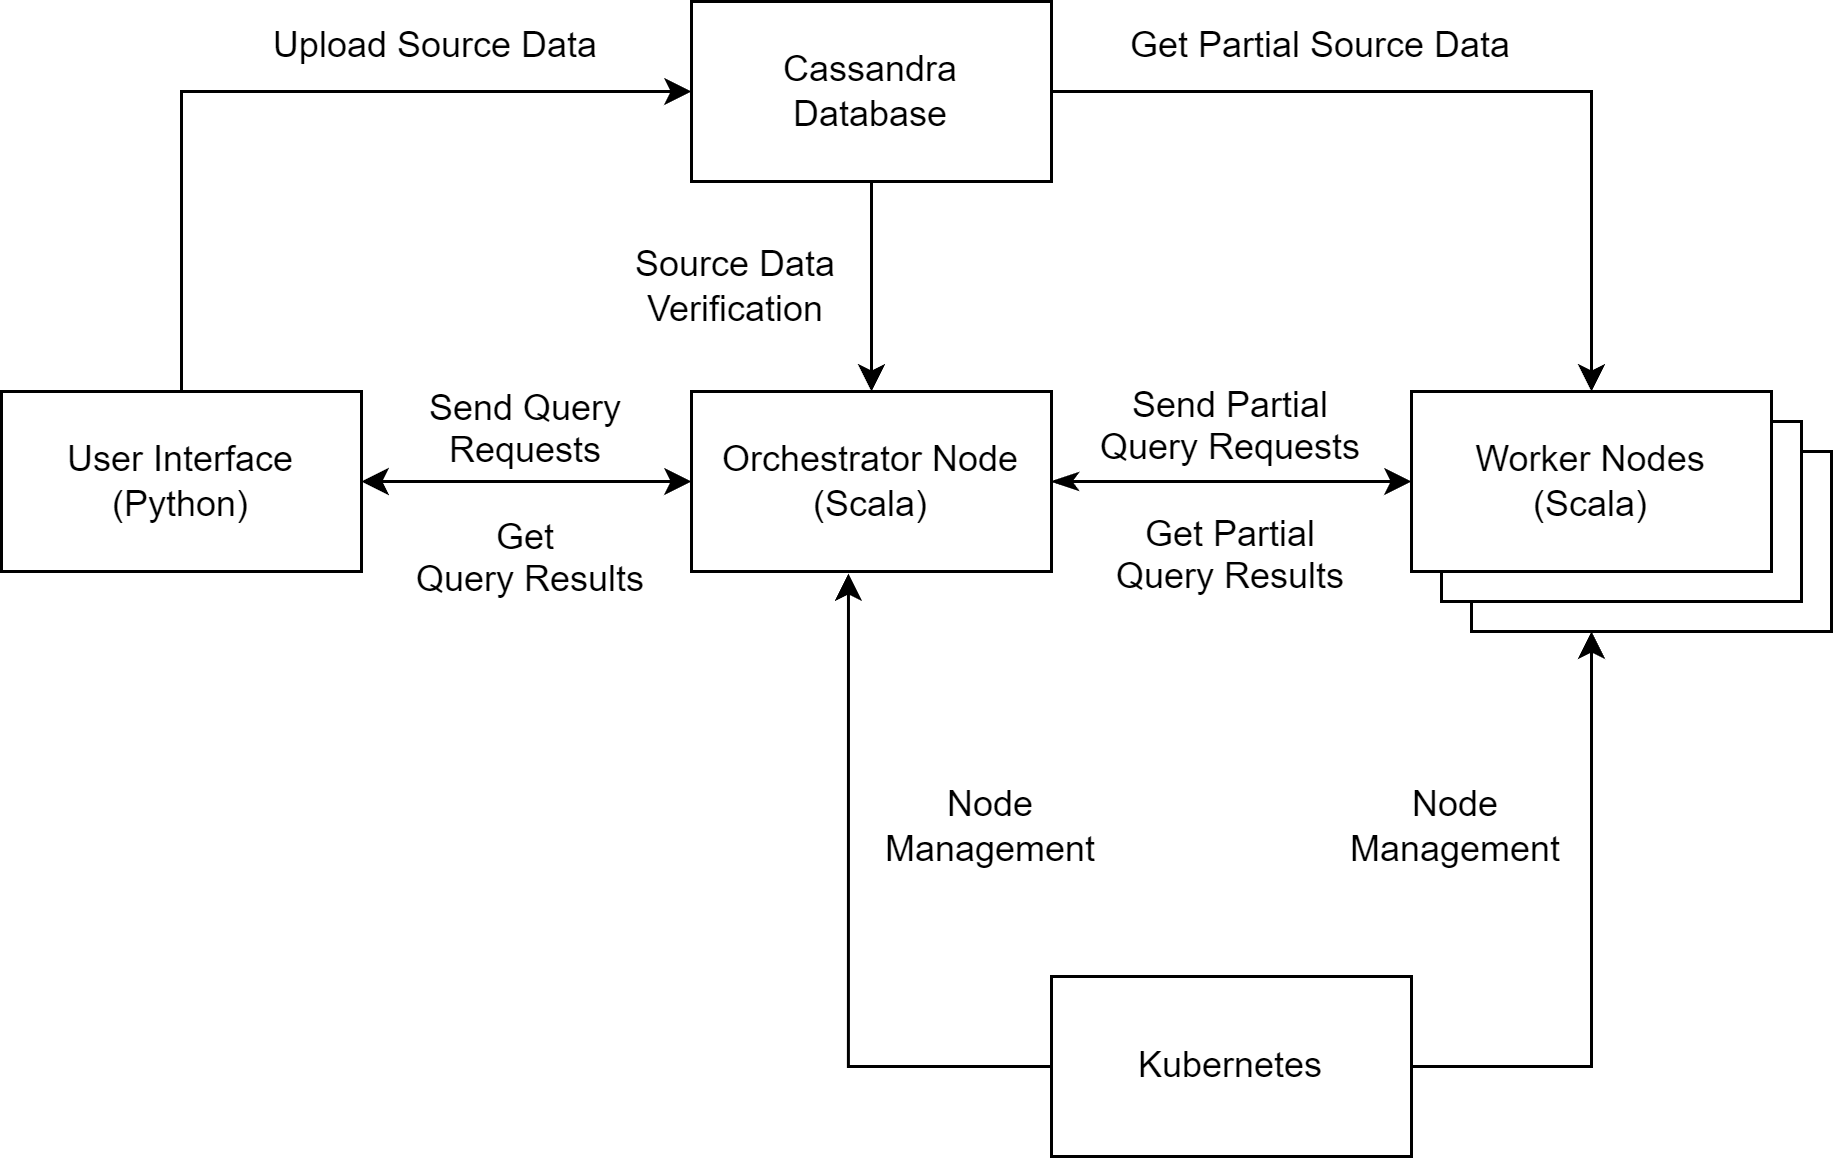
\includegraphics[width=0.6\textwidth]{chapters/diagrams/design/architecture-overall}
	\caption{Proposed Solution - Overall Architecture}
	\label{fig:overall-architecture}
\end{figure}

